\section{Image Captioning}
\begin{frame}{}
    \LARGE Advanced Computer Vision: \textbf{Image Captioning}
\end{frame}

\begin{frame}[allowframebreaks]{Image Captioning}
    \begin{itemize}
        \item A computer Vision task in which we generate captions for images
    \end{itemize}
    \begin{figure}
    \centering
    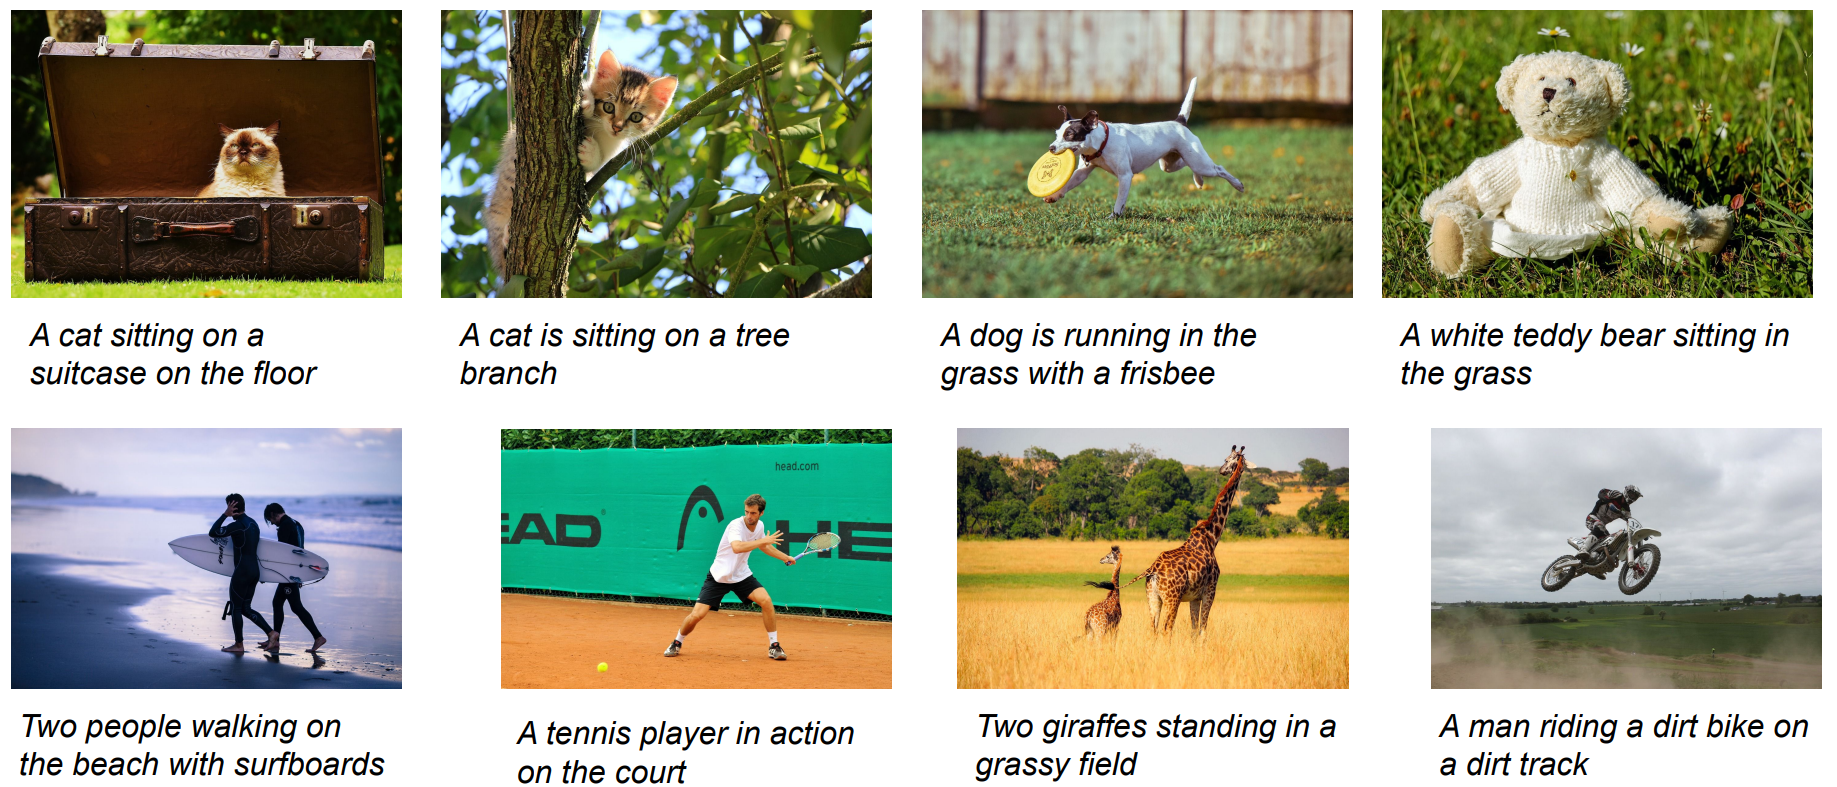
\includegraphics[width=1.0\textwidth,height=1.0\textheight,keepaspectratio]{images/advanced-cv/cap_1.png}
    \end{figure} 

\framebreak
    \begin{itemize}
        \item The task is to generate a natural language description of the content of an image
        \item It combines techniques from computer vision and natural language processing
        \item The process typically involves:
        \begin{itemize}
            \item Extracting features from the image using a convolutional neural network (CNN)
            \item Using these features to generate a sequence of words that describe the image, often with a recurrent neural network (RNN) or transformer model
        \end{itemize}
    \end{itemize}
\framebreak
    \begin{figure}
        \centering
        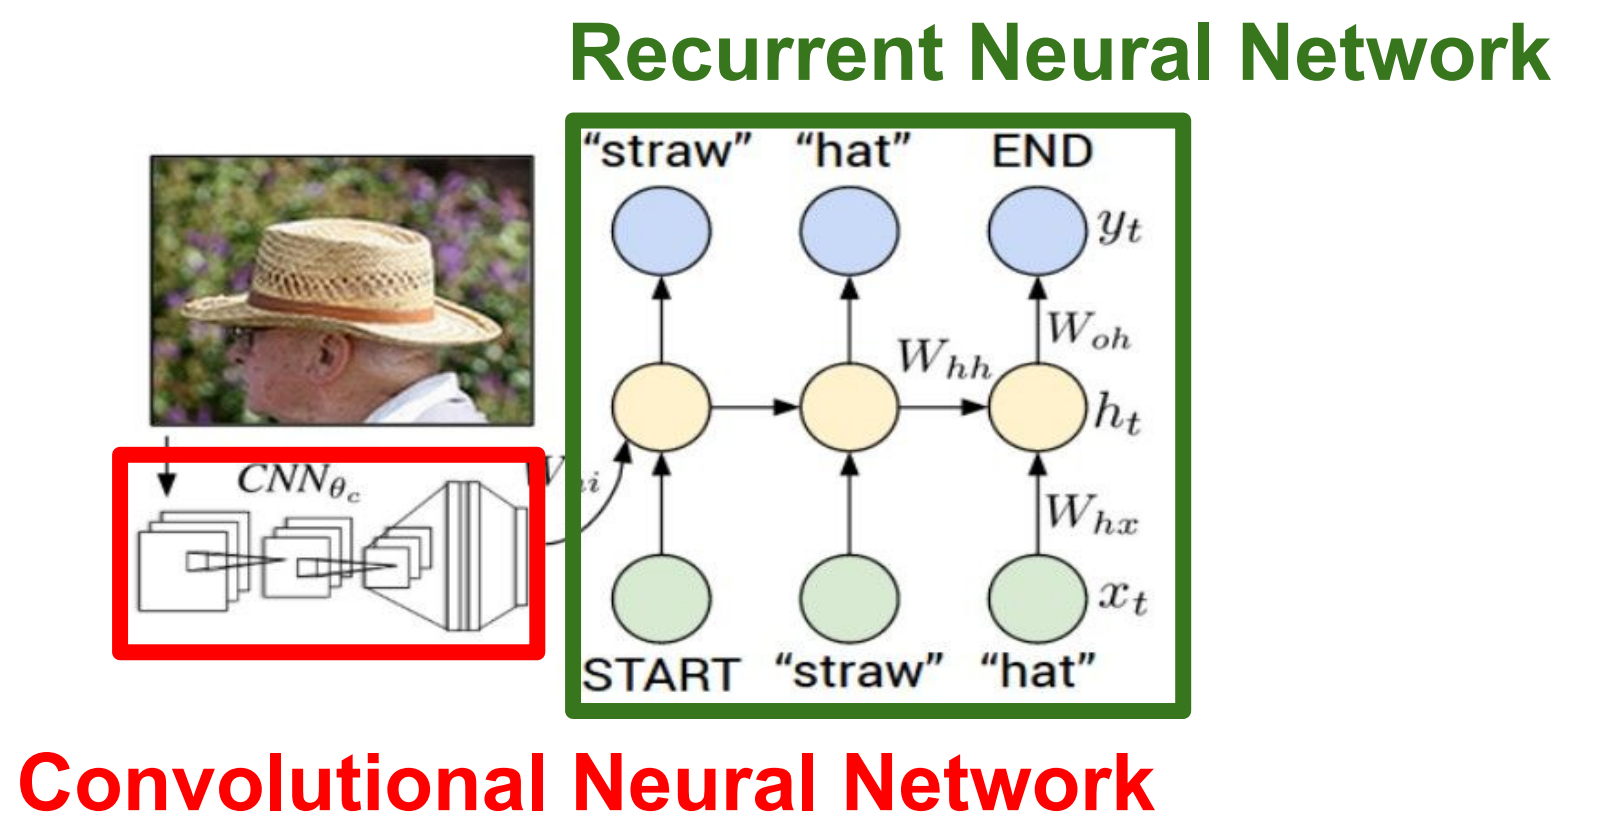
\includegraphics[width=1.0\textwidth,height=1.0\textheight,keepaspectratio]{images/advanced-cv/cap_2.png}
    \end{figure}  
\end{frame}